% =====================================================================
% SUPPLEMENTARY NOTE 7 — the claims axis, protocol by protocol.
%
% SOURCES. The ledger is Paper_writing/CLAIMS_LEDGER.md, built from the
% ten corpus papers' own PDFs; the protocols are EXPERIMENTS.md; every
% number in a table below is read from axw1008/docs/paper/x*.csv or the
% X3 run log by figures/scripts/supp_figures.py. Nothing here is a new
% calculation; it is the existing results laid out so each test can be
% read against the claim it answers.
%
% REGISTER PASS, 15 November, per SUPPLEMENTARY_REGISTER.md. Subsections
% are now the QUESTIONS rather than the X numbers, which mean nothing
% outside EXPERIMENTS.md. The X numbers are kept in the ledger's third
% column so the protocols can still be traced.
% =====================================================================

\section{The claims axis, protocol by protocol}
\label{note:claims}

Eleven studies were pooled to build this atlas, and ten of them made claims
about endometriosis from their own cohorts. None of the ten could test
another's, because no two share donors or a cell vocabulary. Our claims
axis asks which of those claims the pooled corpus can settle, and settles
the ones it can. In this note we give the ledger of claims, then each test
as a protocol with its full table, in the order the tests depend on one
another. The label transfer that every composition test rests on is set out
under \emph{Beyond two studies the cell families are predictions} in
\ref{note:limitations}.

\subsection{The ledger}

Table~\ref{stab:ledger} lists every claim that bears on the disease, with
the cohort it was made from, the test we applied and the outcome. We took
the claims from the papers themselves and not from any review of them.
Three kinds of claim fall outside the axis and we list them so the boundary
is visible: claims about cell types finer than the four families, which
would need a finer transferred vocabulary; claims at the resolution of a
single pathway, which our forty-four groups merge
(\ref{note:limitations}); and claims from the one cohort
whose controls are not in the corpus. On the second of those, the
constraint is the merge and not the size of what was merged: across the
forty-four groups, how many genes a group holds predicts neither what it
carries about cell family, Spearman $-0.058$ at $P = 0.71$, nor what it
carries about the menstrual cycle, $+0.130$ at $P = 0.40$. A claim about
glycolysis cannot be put to a group that merges glycolysis with fifteen
other pathways, and splitting that group into smaller ones would not on its
own make it answerable.

\begin{table}[p]
\centering
\caption[The claims ledger]{\textbf{Published claims about endometriosis
from the corpus studies, and what the pooled corpus does with each.} Donor
counts are the cohort the claim was made from and the donors the test here
used.}
\label{stab:ledger}
\footnotesize\setlength{\tabcolsep}{3pt}
\begin{tabular}{@{}p{40mm}p{30mm}p{38mm}p{44mm}@{}}
\toprule
claim & source, donors & test here, donors & outcome \\
\midrule
eutopic endometrium of patients is transcriptionally altered & \texttt{duempelmann\_2026}, 60;\newline \texttt{tan\_2022}, 31 & cross-donor disease agreement, 207 donor records & supported: 0.3364, $P = 0.005$ \\
composition barely differs between patients and controls once phase is accounted for & \texttt{duempelmann\_2026}, 60 & X8, per-donor composition, 194 & supported: no family moves, $P \geq 0.24$ \\
severity is a dose: severe disease gives five times the differentially expressed genes of mild & \texttt{duempelmann\_2026}, 60 & latent severity among patients, 57; composition among patients, 51 & not recoverable at this donor count, in either readout; a different quantity, not a contradiction \\
macrophages and decidualised stromal cells are the compartments most likely dysregulated & \texttt{marecko\_2024}, 58,\newline from GWAS & X12, held-out disease direction within each family, 85 to 114 & immune half supported, 0.7084 at $P = 0.015$; stromal half not recoverable, 0.5920 at $P = 0.175$ \\
prior atlases lack reproducible marker signatures & \texttt{marecko\_2024} & X13, below & not supported on the marker half: 61 to 76 of each family's top hundred reproduce \\
disease abolishes the cyclical variation of immune composition & \texttt{lin\_2023}\newline (Huang), 13 & X3, cycle agreement by disease, 112; X3b, phase-by-disease interaction on composition, 101 & not supported in either test \\
composition differs between lesion and eutopic tissue & \texttt{ferrero\_2024}\newline (Sarsenova), 4 pairs & X9, per-donor composition by tissue, 151 & one family moves, epithelial 6.6-fold lower, confounded with dissociation; perivascular not resolvable \\
the same cell type differs transcriptionally by tissue site & \texttt{fonseca\_2023}, 48 & X14, tissue within a transferred family, 262 & weak residue in stromal and endothelial, $P = 0.08$ and $0.10$; tissue is a decoder covariate \\
lesions carry a less differentiated, progenitor-like epithelium & \texttt{garcia\_alonso\_2021}\newline (bulk deconvolution);\newline \texttt{tan\_2022}, 14 & needs epithelial subtypes & not tested; 58 ectopic donors available \\
four case-against-control findings, two at $P < 10^{-16}$ & \texttt{shih\_2022}, 11 here & none possible & untestable: no controls in the deposited cohort \\
metabolic reprogramming in named pathways; steroid signalling; iron and senescence & \texttt{ferrero\_2024};\newline \texttt{li\_2025} & needs single-pathway resolution & not tested; the groups merge the pathways named \\
perivascular and mural cell findings in three cohorts & \texttt{duempelmann\_2026},\newline \texttt{tan\_2022},\newline \texttt{ferrero\_2024} & needs a finer vocabulary & future work \\
\bottomrule
\end{tabular}
\end{table}

\subsection{Does disease flatten the menstrual cycle? The latent}

The claim is that in controls the proportions of immune cells vary across
the menstrual cycle and in endometriosis that variation disappears
\citep{huang2023immune}, made from thirteen donors. To ask it of the
latent, we computed cross-donor cycle agreement separately over control
donors and over eutopic donors, and built a permutation null for the
difference by reassigning disease status across donors.

We dropped the held-out restriction for this test. The phase head is one
linear map from latent position to phase and cannot store which donor had
which phase, and training donors scored no higher than held-out ones,
0.6422 against 0.6545. Keeping the restriction would have cost two thirds
of the donors for nothing.

Over 112 donors the control excess is 0.6825 and the eutopic 0.7474, a
difference of $-0.0650$ against a null spanning $-0.1802$ to $+0.1949$,
$P = 0.505$ (Tables~\ref{stab:x3} and~\ref{stab:x3d}). The claim predicts a
positive difference. The measured one is small and negative, and the null
is narrow enough that a difference of the size claimed would have been
seen. Phase labels come from three studies, so this is a three-cohort
result and not a corpus-wide one.

\begin{table}[t]
\centering
\caption[X3, cycle agreement by disease]{\textbf{Cross-donor cycle
agreement among control donors and among eutopic donors.}}
\label{stab:x3}
\small
% GENERATED by figures/scripts/supp_figures.py. Do not edit by hand.
\begin{tabular}{@{}lrrrrrr@{}}
\toprule
donors & n & cells & phases & agreement & chance & excess \\
\midrule
control & 61 & 307{,}040 & 8 & 0.7600 & 0.2443 & 0.6825 \\
eutopic & 51 & 318{,}936 & 6 & 0.8052 & 0.2288 & 0.7474 \\
\bottomrule
\end{tabular}

\end{table}

\begin{table}[t]
\centering
\caption[X3, the difference and its null]{\textbf{The difference between
the two groups and its permutation null.}}
\label{stab:x3d}
\small
% GENERATED by figures/scripts/supp_figures.py. Do not edit by hand.
\begin{tabular}{@{}lr@{}}
\toprule
quantity & value \\
\midrule
control minus eutopic, excess & $-$0.0650 \\
null mean & 0.0018 \\
null s.d. & 0.0961 \\
null 95\% interval & $-$0.1802 to 0.1949 \\
two-sided $P$ & 0.505 \\
permutations & 2{,}000 \\
\bottomrule
\end{tabular}

\end{table}

\subsection{Does disease flatten the menstrual cycle? The proportions}

The claim is about proportions and not about latent geometry, so our second
test uses no model output. For each of 101 donors carrying a family label,
a phase and a disease status, we fitted the immune share of cells as
$\mathrm{logit}(\text{share}) \sim \text{study} + \text{phase} +
\text{disease} + \text{phase} \times \text{disease}$. The interaction term
is the claim written as arithmetic. Our null permutes disease status across
donors within study, keeping each donor's phase and composition together,
5{,}000 times.

The interaction $F$ is 0.263 against a null whose 95th percentile is 3.061,
$P = 0.762$ (Table~\ref{stab:x3b}). Thus the two tests use different
instruments, one the representation and one a headcount, and they agree.
The second cannot be attributed to anything the model does.

\begin{table}[t]
\centering
\caption[X3b, the interaction test]{\textbf{The phase-by-disease interaction
on immune composition}, 101 donors, study as a covariate.}
\label{stab:x3b}
\small
% GENERATED by figures/scripts/supp_figures.py. Do not edit by hand.
\begin{tabular}{@{}lr@{}}
\toprule
quantity & value \\
\midrule
donors & 101 \\
interaction $F$, phase $\times$ disease & 0.263 \\
null mean $F$ & 0.996 \\
null 95th percentile & 3.061 \\
$P$ & 0.762 \\
permutations & 5{,}000 \\
\bottomrule
\end{tabular}

\end{table}

\subsection{Does composition differ between lesion and endometrium?}

The claim is that perivascular, endothelial and immune cells form a larger
share of lesions and stromal cells a smaller one
\citep{sarsenova2024metabolic}, from four paired samples. For each of 151
donors we computed the share of each family over the transferred and
annotated labels together, then tested eutopic endometrium against lesion
tissue after study, with a permutation null of 5{,}000 reassignments within
study. One caution about the shape of that test: the four shares sum to
one and we named the families in advance, so these are not four
independent attempts.

One family moves. The epithelial share falls from 0.147 in eutopic
endometrium to 0.022 in lesion tissue, 6.6-fold, $F = 20.9$, $P < 0.0001$,
and immune, endothelial and stromal do not clear
(Table~\ref{stab:x9}, Supplementary Fig.~\ref{sfig:comp-ee}). The direction
agrees with the claim. However, the source names the confound: epithelial
cells are lost when fibrous lesion tissue is dissociated, and nothing in
the corpus separates that from biology. The label absorption of
\ref{note:limitations} would push the epithelial share in lesions up and not
down, so it does not manufacture this result.
Perivascular cells are not one of our four families, so the claim's central
compartment stays out of reach.

\begin{table}[t]
\centering
\caption[X9, composition by tissue]{\textbf{Per-donor cell-family share,
eutopic endometrium against lesion tissue}, 151 donors.}
\label{stab:x9}
\small
% GENERATED by figures/scripts/supp_figures.py. Do not edit by hand.
\begin{tabular}{@{}lrrrr@{}}
\toprule
family & mean share, eutopic & mean share, ectopic & $F$ & $P$ \\
\midrule
stromal & 0.584 & 0.496 & 0.044 & 0.8180 \\
epithelial & 0.147 & 0.022 & 20.895 & $<$ 0.0001 \\
endothelial & 0.039 & 0.080 & 0.208 & 0.7002 \\
immune & 0.230 & 0.401 & 2.864 & 0.1194 \\
\bottomrule
\end{tabular}

\end{table}

\begin{figure}[t]
\centering
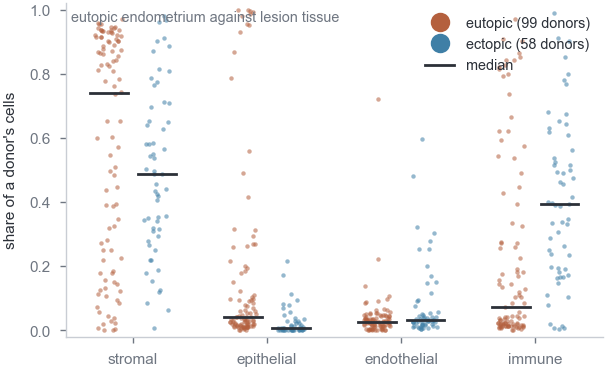
\includegraphics[width=.65\textwidth]{figures/composition_eutopic_vs_ectopic.png}
\caption[Composition, eutopic against lesion]{\textbf{One family of four
separates lesion tissue from eutopic endometrium, and it is the one the
source study names a dissociation artefact.} Each donor's share of each
cell family over the transferred and annotated labels together, eutopic
endometrium against lesion tissue, 151 donors, bars at the medians. The
epithelial share falls from a mean of 0.147 to 0.022, a 6.6-fold drop at
$F = 20.9$ and $P < 0.0001$ after study. Stromal, endothelial and immune do
not clear, at $P = 0.8180$, 0.7002 and 0.1194, although the immune mean
nearly doubles from 0.230 to 0.401. The four shares sum to one and the
families were named in advance, so these are not four independent
attempts. Perivascular cells, the compartment the claim is actually about,
are not one of the four families and stay out of reach.}
\label{sfig:comp-ee}
\end{figure}

\subsection{Where in the latent does the disease live?}

The claim is that macrophages and decidualised stromal cells are the
compartments most likely dysregulated in endometriosis, derived by
integrating an atlas with the largest endometriosis GWAS
\citep{mareckova2024heca}. To test it we looked for a direction in the
latent separating control donors from eutopic donors, fitting on 70\% of
donors and scoring by AUC on the remaining 30\%, repeated over 400
donor-level splits with a shuffled-label null. We centred study out and
used donors rather than cells as the units.

Globally no such direction exists: 0.5360 against a shuffled 0.4820 over
207 donor records, with 28\% of shuffles above it
(Table~\ref{stab:x12g}). That does not contradict our cross-donor disease
figure, which is local. A cell's neighbours from other donors can share its
label without any single axis separating the donors.

Inside each family, over the 118 donors with the studies' own labels, the
direction appears and it is immune: AUC 0.7084 against 0.4806,
$P = 0.015$ over 94 donors; endothelial 0.6818 at $P = 0.050$; stromal
0.5920 at 0.175; epithelial 0.4663 at 0.590; and the four families pooled
0.6048 at 0.155 (Table~\ref{stab:x12a},
Supplementary Fig.~\ref{sfig:x12-auc-a}). Mixing the families destroys a
signal that is present inside one of them. We tested four families, so a
Bonferroni correction puts immune at about 0.06 and endothelial at 0.20,
and immune is the only compartment worth calling real rather than
emphatic. On the transferred labels over 207 donor records the pattern
holds and weakens, immune 0.5960 at $P = 0.072$ over 162
(Table~\ref{stab:x12t}, Supplementary Fig.~\ref{sfig:x12-auc-t}). Our
reason for reporting 118 rather than 207 is given in
\ref{note:limitations}.

\begin{table}[t]
\centering
\caption[X12, the global direction]{\textbf{The global control-against-case
direction}, fitted and scored across donor-level splits.}
\label{stab:x12g}
\small
% GENERATED by figures/scripts/supp_figures.py. Do not edit by hand.
\begin{tabular}{@{}lr@{}}
\toprule
quantity & value \\
\midrule
donor records & 207 \\
held-out AUC, global direction & 0.5360 \\
shuffled-label AUC & 0.4820 \\
share of shuffles above observed & 0.28 \\
cosine stability of the direction across splits & 0.8526 \\
\bottomrule
\end{tabular}

\end{table}

\begin{table}[t]
\centering
\caption[X12, direction within each family, own labels]{\textbf{The
disease direction within each family, studies' own labels}, 118 donors.
Interval is the 2.5th to 97.5th percentile over 400 splits.}
\label{stab:x12a}
\footnotesize
% GENERATED by figures/scripts/supp_figures.py. Do not edit by hand.
\begin{tabular}{@{}lrrrrrr@{}}
\toprule
compartment & donors & ctl / case & held-out AUC & 95\% interval & shuffled AUC & $P$ \\
\midrule
all families, pooled & 114 & 60 / 54 & 0.6048 & 0.454 to 0.750 & 0.5028 & 0.155 \\
stromal & 101 & 54 / 47 & 0.5920 & 0.437 to 0.753 & 0.4986 & 0.175 \\
epithelial & 98 & 51 / 47 & 0.4663 & 0.304 to 0.632 & 0.4898 & 0.590 \\
immune & 94 & 50 / 44 & 0.7084 & 0.566 to 0.856 & 0.4806 & 0.015 \\
endothelial & 85 & 43 / 42 & 0.6818 & 0.523 to 0.827 & 0.4864 & 0.050 \\
\bottomrule
\end{tabular}

\end{table}

\begin{table}[t]
\centering
\caption[X12, direction within each family, transferred labels]{\textbf{The
same test over 207 donor records with transferred labels.}}
\label{stab:x12t}
\footnotesize
% GENERATED by figures/scripts/supp_figures.py. Do not edit by hand.
\begin{tabular}{@{}lrrrrrr@{}}
\toprule
compartment & donors & ctl / case & held-out AUC & 95\% interval & shuffled AUC & $P$ \\
\midrule
all families, pooled & 202 & 106 / 96 & 0.5176 & 0.411 to 0.624 & 0.4710 & 0.268 \\
stromal & 175 & 86 / 89 & 0.4921 & 0.379 to 0.610 & 0.4804 & 0.445 \\
epithelial & 176 & 93 / 83 & 0.4701 & 0.338 to 0.581 & 0.4780 & 0.535 \\
immune & 162 & 76 / 86 & 0.5960 & 0.471 to 0.711 & 0.4821 & 0.072 \\
endothelial & 134 & 65 / 69 & 0.5947 & 0.481 to 0.709 & 0.4782 & 0.102 \\
\bottomrule
\end{tabular}

\end{table}

\begin{figure}[t]
\centering
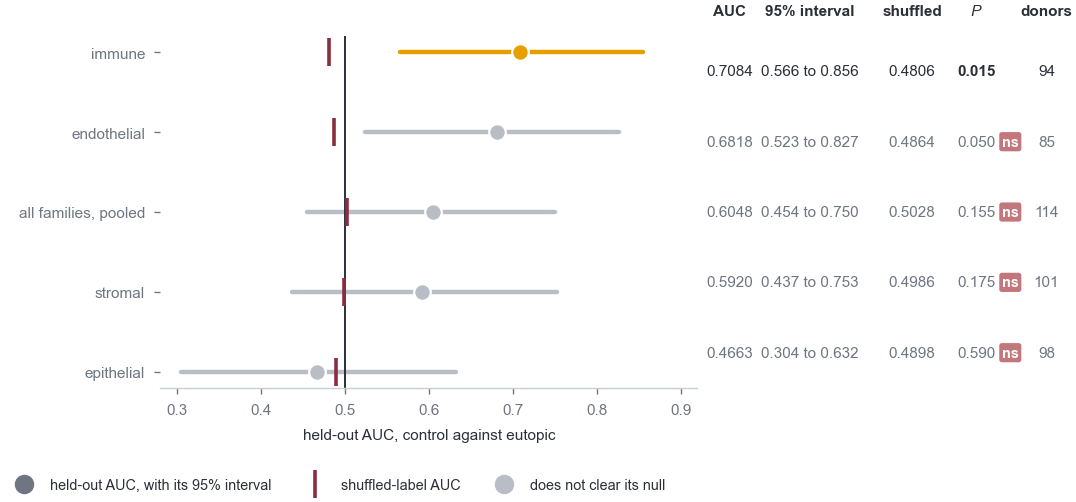
\includegraphics[width=\textwidth]{figures/x12_auc_by_family_annotated.png}
\caption[Disease AUC by family, own labels]{\textbf{Pooling the four
families destroys a disease direction that is legible inside the immune
compartment alone.} Held-out area under the receiver operating
characteristic curve (AUC) for a direction separating control from eutopic
endometrium, fitted within each cell family and over all four pooled,
using only the two studies that annotated their own cells. Circles are the
held-out AUC with its 95\% interval; the dark tick is the same procedure
on shuffled labels; rows that do not clear their null are greyed and
badged ns, and the aligned columns give every value including the donor
count. Immune reaches 0.7084 against a shuffled 0.4806 at $P = 0.015$ over
94 donors. Pooling the families falls to 0.6048 at $P = 0.155$ over a
larger 114, so the loss is not a loss of donors, and epithelial cells
carry nothing at 0.4663. Endothelial sits at exactly $P = 0.050$, which is
why this figure prints every $P$ rather than replacing it with a badge.}
\label{sfig:x12-auc-a}
\end{figure}

\begin{figure}[t]
\centering
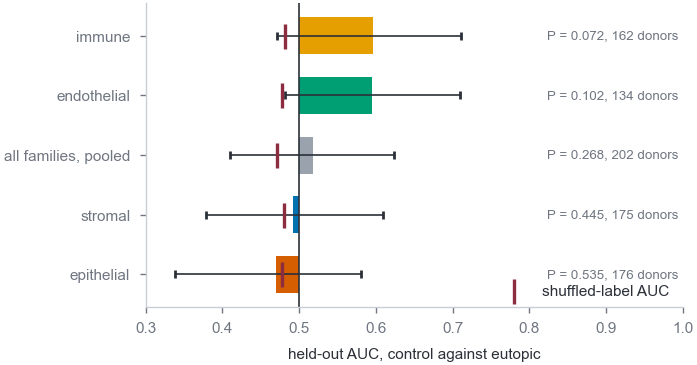
\includegraphics[width=\textwidth]{figures/x12_auc_by_family_transferred.png}
\caption[Disease AUC by family, transferred labels]{\textbf{The same test
over nearly twice the donors, on transferred labels, and nothing clears
its null.} Layout and procedure as in
Supplementary Fig.~\ref{sfig:x12-auc-a}, run over 207 donor records whose
cell families come from the nearest-neighbour transfer rather than from a
study's own annotation. Immune remains the strongest compartment and keeps
its sign, 0.5960 against a shuffled 0.4821 at $P = 0.072$ over 162 donors,
but it does not strengthen with scale, and the pooled contrast falls to
0.5176. Two explanations are not separable here: transferred labels add
noise, or the nine added studies are heterogeneous in ways the two
annotated ones are not. Neither this figure nor
Supplementary Fig.~\ref{sfig:x12-auc-a} should be quoted alone.}
\label{sfig:x12-auc-t}
\end{figure}

\subsection{Which genes does the immune direction move?}

To name the genes behind that direction, we pushed it through the decoder.
We moved 4{,}000 immune cells along it and recorded the change in every one
of the 15{,}496 decoded genes, after removing the component of the
direction lying along the family axes. The ranking is stable in the step
size, with a rank correlation of 0.9973 between two step lengths.

Table~\ref{stab:x12top} gives the fifteen genes that move most towards
disease and Table~\ref{stab:x12bot} the fifteen that move most towards
control. Supplementary Fig.~\ref{sfig:x12-rank} draws the whole ranking.
The disease end is macrophage and inflammatory transcripts, TREM1, IL1B,
CCL13, SIGLEC7, the matrix proteases MMP19 and MMP27, LRRC15 and INHBA,
with CCL3 at rank 52 and ITGAX at 47 just outside the table.

Three external readings bear on it. An independent cohort outside the
corpus, eight patients against five controls, published 66 genes
upregulated in the eutopic endometrium of patients
\citep{zhao2017transcriptome}. Four of our fifteen disease-end genes are on
that list, SERPINB2 at 72.95-fold, MMP27 at 40.93, LRRC15 at 25.20 and
INHBA at 15.33, a hypergeometric $P$ of $3.95 \times 10^{-7}$ for fifteen
draws from 15{,}496, and none of our fifteen control-end genes is on it at
all. In addition, IL1B, tenth here, is the
highest-ranked gene in \texttt{duempelmann\_2026}'s own supervised
classifier of disease, so two models with different objectives select it,
and CCL3 and ITGAX appear in that cohort's ligand-receptor findings as well
\citep{duempelmann2026endometrium}. Of the four gene-level predictions of
the prior atlas, only IGF1 rising in macrophages is a claim about this
compartment, and it agrees, at rank 285 of 15{,}496 towards disease. GREB1,
DKK1 and IGF2 are predictions about decidualised stromal cells, and there
is no stromal direction to test them on.

A larger bulk cohort does not bear on the direction either way: in
EndometDB, 62 patient against 38 control endometria
\citep{gabriel2020endometdb}, no gene differs at FDR 0.05, and our ranking
is essentially uncorrelated with its patient-control statistic (Spearman
$\rho = -0.052$; $+0.037$ in untreated women).

Two cautions attach to the ranking. The control end is led by genes of
epithelial identity and secretory function, VTCN1, SOX17, IHH and UGT2B17,
with WNT7A, LGR5, MSLN and TFF3 inside the last 220. We do not read that
end as disease biology and it replicates nothing. Separately, four of the
fifteen disease-end genes, SIGLEC7, ADAMDEC1, ALPK2 and KCNH1, have no
prior endometriosis report in the eleven pooled studies, the Open Targets
Platform or PubMed. Two of the genes that do replicate, LRRC15 and MMP27,
are absent from one or both of those indices despite being reported at 25-
and 41-fold in the external cohort's supplementary tables. Thus absence
from an index is not evidence of novelty, and we report the four as
unindexed.

\begin{table}[p]
\centering
\caption[X12, the disease end of the ranking]{\textbf{The fifteen genes
moving most towards disease along the immune direction.}}
\label{stab:x12top}
\footnotesize
% GENERATED by figures/scripts/supp_figures.py. Do not edit by hand.
\begin{tabular}{@{}rlrrl@{}}
\toprule
rank & gene & shift towards disease & external up-list, fold & indexed report \\
\midrule
1 & LRRC15 & 0.0733 & 25.20 &  \\
2 & TREM1 & 0.0620 & -- &  \\
3 & SCARA5 & 0.0616 & -- &  \\
4 & CCL13 & 0.0608 & -- &  \\
5 & CST11 & 0.0606 & -- &  \\
6 & SIGLEC7 & 0.0594 & -- & none found \\
7 & KCNH1 & 0.0592 & -- & none found \\
8 & DKK1 & 0.0571 & -- &  \\
9 & SERPINB2 & 0.0569 & 72.95 &  \\
10 & IL1B & 0.0567 & -- &  \\
11 & MMP19 & 0.0566 & -- &  \\
12 & MMP27 & 0.0559 & 40.93 &  \\
13 & ADAMDEC1 & 0.0556 & -- & none found \\
14 & INHBA & 0.0555 & 15.33 &  \\
15 & ALPK2 & 0.0550 & -- & none found \\
\bottomrule
\end{tabular}

\end{table}

\begin{table}[p]
\centering
\caption[X12, the control end of the ranking]{\textbf{The fifteen genes
moving most towards control along the same direction.}}
\label{stab:x12bot}
\small
% GENERATED by figures/scripts/supp_figures.py. Do not edit by hand.
\begin{tabular}{@{}rlr@{}}
\toprule
rank & gene & shift towards control \\
\midrule
1 & PLP1 & 0.0670 \\
2 & AMIGO3 & 0.0644 \\
3 & INS & 0.0622 \\
4 & UGT1A5 & 0.0598 \\
5 & NPY2R & 0.0581 \\
6 & SLIT2 & 0.0578 \\
7 & CFHR4 & 0.0577 \\
8 & NPAP1 & 0.0547 \\
9 & DCLK1 & 0.0539 \\
10 & EPHA5 & 0.0533 \\
11 & EBF2 & 0.0531 \\
12 & ADGRB3 & 0.0525 \\
13 & LRRC15 & 0.0523 \\
14 & COL6A6 & 0.0519 \\
15 & HTN1 & 0.0517 \\
\bottomrule
\end{tabular}

\end{table}

\begin{figure}[t]
\centering
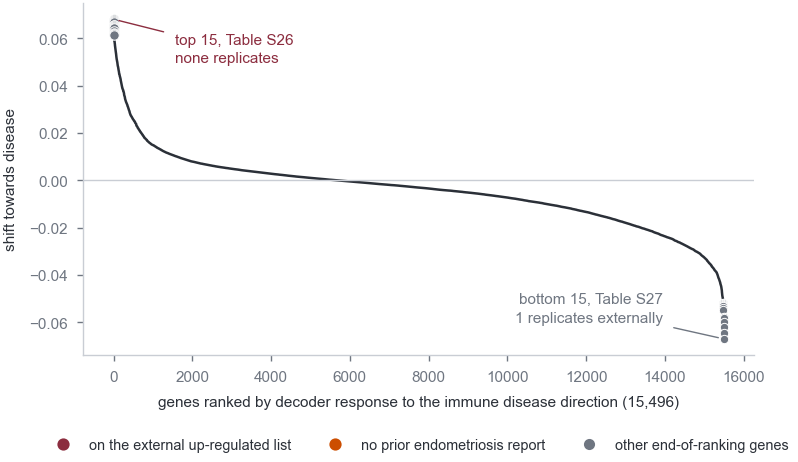
\includegraphics[width=.9\textwidth]{figures/x12_gene_ranking.png}
\caption[The gene ranking along the immune direction]{\textbf{The decoder's
response is flat across fourteen thousand genes and turns hard at both
ends, and only one of those ends replicates externally.} All 15{,}496
genes ranked by the decoder's response to the immune disease direction,
with the top fifteen and bottom fifteen marked. Colour at the disease end
separates the four genes on an external cohort's 66-gene upregulated list,
SERPINB2, MMP27, LRRC15 and INHBA, from the four with no prior
endometriosis report in the eleven pooled studies, the Open Targets
Platform or PubMed, SIGLEC7, ADAMDEC1, ALPK2 and KCNH1. The gene names are
in Tables~\ref{stab:x12top} and~\ref{stab:x12bot} and are not repeated
here. Four hits from fifteen draws out of 15{,}496 against a 66-gene list
carries a hypergeometric $P = 3.95 \times 10^{-7}$; the control end of the
same ranking, drawn the same way against the same list, returns none.}
\label{sfig:x12-rank}
\end{figure}

\subsection{Does tissue separate cells within one family?}

The claim is that the same cell type is transcriptionally different
depending on the tissue it sits in \citep{fonseca2023endometriosis}.
Tissue is a decoder covariate, which conditions the test rather than
invalidating it. Conditioning the decoder on tissue removes the latent's
obligation to encode it, so tissue structure that survives in the latent is
structure the model had every reason to discard. Within each transferred
family we scored (donor, tissue) units for endometrium against lesion
tissue after study, 262 donors, with donor-level splits and a shuffled
null.

Most tissue structure is gone. What remains sits in stromal and endothelial
cells, AUC 0.6226 at $P = 0.077$ and 0.6175 at 0.095, with immune and
epithelial at chance (Table~\ref{stab:x14},
Tissue is near-perfectly confounded
with disease status here, since ovary and peritoneum are almost all ectopic
donors. This is therefore the latent-level companion to the lesion
composition test above and not an independent axis, and neither family
clears 0.05.

\begin{table}[t]
\centering
\caption[X14, tissue within a family]{\textbf{Endometrium against lesion
tissue within each transferred family}, 262 donors.}
\label{stab:x14}
\small
% GENERATED by figures/scripts/supp_figures.py. Do not edit by hand.
\begin{tabular}{@{}lrrrrrr@{}}
\toprule
family & (donor, tissue) units & endometrium & lesion & AUC & shuffled AUC & $P$ \\
\midrule
stromal & 229 & 171 & 58 & 0.6226 & 0.4946 & 0.077 \\
epithelial & 194 & 173 & 21 & 0.5222 & 0.4936 & 0.401 \\
endothelial & 175 & 131 & 44 & 0.6175 & 0.4935 & 0.095 \\
immune & 215 & 158 & 57 & 0.5618 & 0.5019 & 0.240 \\
\bottomrule
\end{tabular}

\end{table}

\subsection{Do marker signatures reproduce across cohorts?}

The largest prior atlas of the endometrium states that earlier atlases lack
reproducible marker gene signatures, consensus annotation, and even cycle
coverage \citep{mareckova2024heca}. We can test the marker half of that
claim here and in no single cohort, because testing it needs independently
annotated cohorts measured on one gene space, which is what the pooled
corpus is. It is also the one test in this axis that uses the count
matrices and the studies' own annotations and never touches the model, so
it is a statement about the corpus and not about \elaj{}.

Two studies annotated their own cells at the family level,
\texttt{duempelmann\_2026} with 132{,}259 held-out cells and
\texttt{marecko\_2024} with 44{,}544, each labelling stromal, epithelial,
endothelial and immune. Within each study and for each family, we derived a
one-against-rest signature over every gene that study measured: the
standardised mean difference, on log-transformed counts per ten thousand,
between the family's cells and the rest of that study's cells. The
statistic is deterministic, runs in two sparse passes, and is monotone in
the $t$-statistic a marker ranking would use. We used the two studies' own
labels and not the transferred ones, because a signature derived from a
transferred label is a reading of a prediction, and agreement between two
such signatures would partly measure whether the transfer was consistent
rather than whether the biology is.

Specifically, we restricted every comparison to the 13{,}034 genes both
panels measured. A study's panel does not measure every gene in the
vocabulary, and an unmeasured gene arrives as a structural zero. Compared
without the restriction, a gene absent from one panel reads as a confident
non-marker there rather than as unknown, which would depress every
agreement by an amount that depends on how different the two panels are. We
then scored agreement two ways per family: the number of genes shared
between the two studies' top hundred, and the Spearman rank correlation
between the two signatures over all 13{,}034 genes. Our null shuffles
family labels within each study, keeping each study's family proportions,
and reruns the whole comparison twenty times. The overlap of two
top-hundred lists has a floor set by the list length and the gene count,
and the null is what measures that floor.

The two cohorts rank the same genes at the top for every family, sharing 61
to 76 of each other's top hundred at rank correlations from 0.7129 to
0.8256, where twenty within-study label shuffles never share more than
three genes and never leave the interval $-0.048$ to $+0.067$
(Table~\ref{stab:x13}, Supplementary Fig.~\ref{sfig:x13}). Two cohorts that sequenced different people, in
different laboratories, on different platforms, and annotated their cells
independently, agree on what marks a family once they are read on one gene
space. On the marker half of the claim, the signatures reproduce.

Three bounds attach to it. It is one pair of cohorts, because only two
studies in the corpus annotated their own cells. It is four families,
because that is the vocabulary the two share, so whether finer cell types
reproduce as well is not answered here and would need the finer
vocabularies reconciled first. In addition, the restriction to jointly
measured genes is what makes the comparison fair and it is also a choice: a
reader who compares the two cohorts on each study's full panel will find
lower agreement, and that difference is the panels and not the biology. The
other half of the complaint, cycle coverage, applies to this corpus, since
our phase labels come from three studies and a cycle day from one. We quote
the corpus against the claim with that half conceded.

\begin{table}[t]
\centering
\caption[Marker reproducibility by family]{\textbf{Agreement between the
two cohorts' per-family marker signatures, against twenty within-study
label shuffles.} Jaccard is the top-hundred overlap over the union of the
two lists.}
\label{stab:x13}
\footnotesize
\resizebox{\textwidth}{!}{% GENERATED by figures/scripts/supp_figures.py. Do not edit by hand.
\begin{tabular}{@{}lrrrrrr@{}}
\toprule
family & shared genes & top-100 overlap & Jaccard & Spearman $\rho$ & null max overlap & null $\rho$ range (20 shuffles) \\
\midrule
stromal & 13034 & 76 & 0.613 & 0.8256 & 2 & $-$0.036 to +0.046 \\
epithelial & 13034 & 69 & 0.527 & 0.8121 & 3 & $-$0.032 to +0.048 \\
endothelial & 13034 & 69 & 0.527 & 0.7129 & 3 & $-$0.043 to +0.067 \\
immune & 13034 & 61 & 0.439 & 0.8053 & 2 & $-$0.048 to +0.042 \\
\bottomrule
\end{tabular}
}
\end{table}

\begin{figure}[t]
\centering
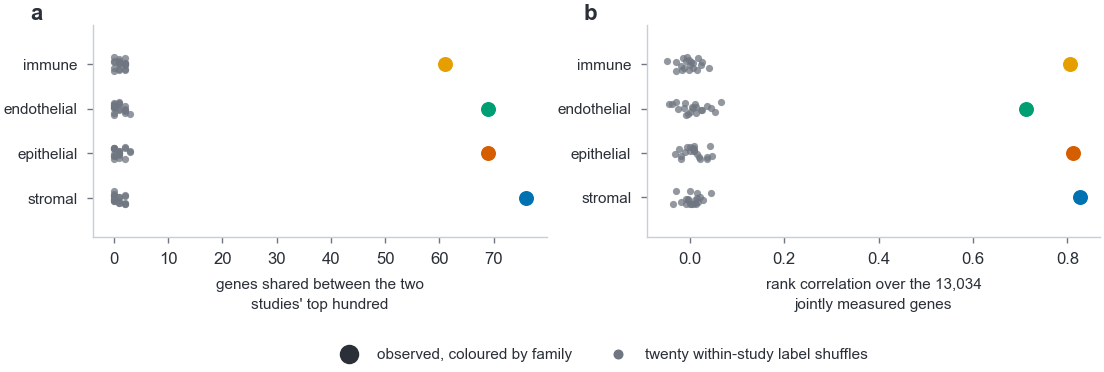
\includegraphics[width=\textwidth]{figures/x13_vs_null.png}
\caption[Marker agreement against the label-shuffled null]{\textbf{The two
cohorts' marker signatures agree far outside anything label shuffling
produces.} Each row is one cell family; coloured points are the observed
agreement between \texttt{duempelmann\_2026} and \texttt{marecko\_2024},
grey points the twenty within-study label shuffles. \textbf{a}, Genes
shared between the two studies' top hundred: 76 stromal, 69 epithelial, 69
endothelial and 61 immune, against a shuffled maximum of three in any
family. \textbf{b}, Spearman rank correlation between the two signatures
over the 13{,}034 genes both panels measure: 0.8256, 0.8121, 0.7129 and
0.8053, against a shuffled range of $-0.048$ to $+0.067$. The shuffles keep
each study's family proportions and rerun the whole comparison, so they
measure the floor that list length and gene count impose rather than
chance alone. Neither panel is a near miss: no family's observed value is
within an order of magnitude of its own null.}
\label{sfig:x13}
\end{figure}

\subsection{What the axis settled}

Overall, of the twelve claims in the ledger we could test eight. Two were
supported at three times the donor count that produced them: composition
not differing between patients and controls, and the immune half of the
dysregulated-compartment prediction. Two were not supported, the cycle
being flattened by disease, tested two ways, and the marker-signature
complaint of the largest prior atlas. One was supported in
direction and is confounded in this corpus, the epithelial depletion in
lesions. Three were not recoverable at this donor count rather than
refuted: the severity dose, the stromal half of the compartment prediction
and the tissue effect within a family. The remaining four need either a
finer cell vocabulary, a finer pathway vocabulary, or controls the
deposited cohort does not contain. Every one of those eight tests was
impossible in any single cohort of the corpus, and performing them is the
function this atlas exists for.
